% ChatTLA: Verifier-Guided Decomposition for TLA+ Specification Generation
% Single-file LaTeX source — paste directly into Overleaf (article class).
\documentclass[11pt]{article}

\usepackage[margin=1in]{geometry}
\usepackage{amsmath, amssymb, amsthm}
\usepackage{booktabs}
\usepackage{microtype}
\usepackage{xcolor}
\usepackage{listings}
\usepackage{graphicx}
\usepackage{enumitem}
\usepackage[hidelinks]{hyperref}
\usepackage{url}
\usepackage{caption}
\usepackage{pgfplots}
\pgfplotsset{compat=1.18}
\usepackage{array}

% --- TLA+ listing style -----------------------------------------------------
\definecolor{kwblue}{RGB}{0,0,180}
\definecolor{cmgray}{RGB}{120,120,120}
\definecolor{strgreen}{RGB}{0,120,0}
\lstdefinelanguage{TLA}{
  morekeywords={MODULE, EXTENDS, VARIABLES, CONSTANT, CONSTANTS, ASSUME,
                THEOREM, LEMMA, PROOF, BY, DEF, DEFS, EXCEPT, IF, THEN, ELSE,
                LET, IN, CASE, OTHER, INSTANCE, LOCAL, EXTENDS, UNCHANGED,
                ENABLED, CHOOSE, SUBSET, UNION, DOMAIN, TRUE, FALSE, BOOLEAN,
                Init, Next, Spec, TypeOK, Inv},
  sensitive=true,
  morecomment=[l]{\\*},
  morecomment=[s]{(*}{*)},
  morestring=[b]",
}
\lstset{
  basicstyle=\ttfamily\footnotesize,
  keywordstyle=\color{kwblue}\bfseries,
  commentstyle=\color{cmgray}\itshape,
  stringstyle=\color{strgreen},
  columns=fullflexible,
  showstringspaces=false,
  breaklines=true,
  frame=single,
  framerule=0.3pt,
  framesep=4pt,
  xleftmargin=6pt,
  xrightmargin=6pt,
  aboveskip=6pt,
  belowskip=6pt,
}

% --- Title ------------------------------------------------------------------
\title{ChatTLA: Verifier-Guided Decomposition for TLA\textsuperscript{+}
Specification Generation}
\author{Eric Spencer\\
\small \textit{(Loyola University Chicago)}\\
\small \texttt{REDACTED-USER@luc.edu}}
\date{April 7, 2026}

\begin{document}
\maketitle

% ---------------------------------------------------------------------------
\begin{abstract}
Large language models can produce TLA\textsuperscript{+} text that parses, but
parsing is a weak signal: a specification can satisfy SANY and TLC while
encoding a state space so degenerate that the model checker has nothing to do.
We introduce the \emph{Diamond gate}, a semantic-validity criterion combining
state-count, invariant non-triviality, and a mutation test, and use it to audit
existing TLA\textsuperscript{+} corpora. Of $484$ specifications previously
collected for fine-tuning OpenAI's open-weight \texttt{gpt-oss:20b} model,
\emph{none} satisfy the Diamond gate; of the $50$ \texttt{ProofGen} examples
in the public \texttt{FM-Alpaca} TLA subset, again \emph{none} pass. We
illustrate the failure modes with worked examples drawn from the corpus
(\S\ref{sec:diamond}): canonical specs pass SANY and TLC but encode
single-state or \texttt{UNCHANGED}-dominated state spaces whose verifier
outcome is invariant under both guard- and invariant-mutations. Treating
verifiers as deterministic reward, we then build a decomposition-based
generation pipeline, adapting the proof-decomposition pattern of
LMGPA from theorem proving to specification authoring
(\S\ref{sec:piecewise}): rather than emitting a full \texttt{.tla} file, the
model produces five small pieces (variables, type invariant, initial state,
next-state relation, safety invariants), each validated incrementally and
retried locally on failure. On a held-out 20-problem benchmark, the same
underlying \texttt{gpt-oss:20b} model improves from $4/20$ TLC-passing
specifications under single-shot generation to $6/20$ under piecewise
generation, and SANY pass rate rises from $7/20$ to $12/20$. The headline
numbers conceal a more interesting structure: piecewise generation
\emph{regresses} on two consensus/transaction problems that single-shot
already passes (Two-Phase Commit, Paxos), and trades them for four new TLC
wins concentrated in scheduling and networking, for a net $+2$ TLC and $+5$
SANY at a $\geq 5\times$ compute multiplier (mean $5.5$ attempts vs.\ $1$). We argue that for
formal-method targets, the productive locus of effort is the verifier reward
shape and the inference procedure, not additional fine-tuning on syntactically
labelled corpora.
\end{abstract}

% ---------------------------------------------------------------------------
\section{Introduction}

TLA\textsuperscript{+}~\cite{lamport2002specifying} is a specification language
designed for the precise statement and machine-checked verification of
concurrent and distributed system properties. Engineers use it to expose subtle
race conditions, consensus liveness violations, and protocol corner cases that
are invisible at the level of code review or unit tests~\cite{newcombe2015use}.
Despite this practical leverage, TLA\textsuperscript{+} adoption is bounded by
authoring cost: writing a useful spec requires both fluency in the notation and
a discipline of thought that few non-specialists possess.

A natural hope is that a sufficiently capable language model could close this
gap, lowering the activation energy for formal specification by translating an
informal English description into a runnable \texttt{.tla} module. The
attractive feature of formal methods, from a machine-learning standpoint, is
that the verifier \emph{is} the reward function: SANY parses, TLC explores, and
either the property holds or a counterexample trace appears. There is no taste,
no ambiguous human label, no preference noise.

In practice this hope has been difficult to realise. A recent systematic
evaluation of $30$ LLMs on natural-language-to-TLA\textsuperscript{+}
generation~\cite{spencer2026canllms} reports at most $26.6\%$ syntactic
correctness and only $8.6\%$ semantic correctness across $2{,}730$ runs,
with semantic successes restricted to a single (progressive) prompting
strategy. Our prior work, alongside several public corpora, has accumulated
hundreds of TLA\textsuperscript{+} specifications labelled ``correct'' on
the basis of SANY and TLC alone. We show
in this paper that this label is dangerously weak: a model fine-tuned to
maximise the SANY/TLC signal converges on a class of specifications that pass
both checkers by being \emph{semantically vacuous}---empty or single-state
state spaces, decorative invariants that constrain nothing,
\texttt{UNCHANGED} guards that suppress all transitions. The model has learned
the grammar of formal verification without the discipline.

We make two contributions:

\begin{enumerate}[leftmargin=1.4em,itemsep=2pt]
\item \textbf{The Diamond gate.} A reproducible semantic-validity criterion
that augments SANY and TLC with state-count, invariant non-triviality, and
mutation testing (\S\ref{sec:diamond}). We use Diamond to audit two public
TLA\textsuperscript{+} corpora and find that, under this criterion, neither
contains a single passing example.

\item \textbf{Piecewise verifier-guided generation.} A decomposition pipeline
in which OpenAI's open-weight \texttt{gpt-oss:20b} emits a
TLA\textsuperscript{+} specification as five short, individually validated
pieces, with structured retry on failure (\S\ref{sec:piecewise}). Without
changing the underlying model weights, this yields a modest but
non-uniform improvement in the rate at which generated specs are
non-trivially TLC-checkable on a held-out benchmark, together with a much
sharper attribution of \emph{which} of the five pieces is the binding
constraint (\S\ref{sec:challenges}).
\end{enumerate}

We use \texttt{gpt-oss:20b} (a general-purpose, not coding-specialised, open
model) throughout the paper as our underlying generator. Naming the
checkpoint matters for context: a coding-specialised 20B would have a
different prior over braces, identifiers, and idioms, and we make no claim
that the gains we report transfer unchanged to such a model.

The narrative is, we hope, slightly uncomfortable in a useful way. The
empirical lesson of the past year of fine-tuning runs reported here is that
\emph{more training data did not help}, and that the apparent gains from
several rounds of preference optimisation were illusory artefacts of a
mis-specified reward. The wins came from looking harder at what the verifier
was actually rewarding, and from re-shaping the inference procedure so that
each verifier query was small enough to be informative.

% ---------------------------------------------------------------------------
\section{Background}
\label{sec:background}

\paragraph{TLA\textsuperscript{+} in one paragraph.} A
TLA\textsuperscript{+} module declares a set of \emph{state variables}, an
\emph{initial-state predicate} \texttt{Init}, and a \emph{next-state relation}
\texttt{Next} written as a disjunction of action formulas relating unprimed
(current) and primed (successor) variables. A separate \emph{invariant} is a
predicate that should hold in every reachable state. The model checker TLC
takes a finite instance (concrete bounds on constants) and exhaustively
explores the reachable-state graph, reporting any violation of an invariant or
deadlock. SANY is the upstream parser/semantic analyser; SANY success is
necessary but not sufficient for a specification to be meaningful.

\paragraph{Why SANY+TLC is not enough.} Consider the (deliberately bad)
specification in Listing~\ref{lst:vacuous}.

\begin{lstlisting}[language=TLA,caption={A SANY- and TLC-passing specification with no semantic content.},label={lst:vacuous}]
---- MODULE Vacuous ----
EXTENDS Naturals
VARIABLES x

TypeOK == x \in Nat

Init == x = 0

Next == UNCHANGED x

SafetyInv == x >= 0
====
\end{lstlisting}

This module parses cleanly. TLC explores its reachable-state graph in less
than a millisecond, finds the single state $x=0$, observes that
\texttt{SafetyInv} holds there, and reports success. By any binary metric
(\texttt{sany\_pass}, \texttt{tlc\_pass}) this is a ``gold'' specification.
It is also useless: the system has no behaviour, the invariant is vacuously
true (it would be true even with the wrong sign), and no bug in any real
implementation could be caught by it.

The pathology generalises. A model trained to maximise binary
\texttt{tlc\_pass} naturally drifts toward
\texttt{Vacuous}-shaped specifications: tighter type bounds make the state
space smaller, \texttt{UNCHANGED} guards make actions ineffective, and weaker
invariants are harder to violate. Each of these moves \emph{increases} the
chance of a green check from the verifier, while \emph{decreasing} the
specification's fidelity to the system being modelled.

\paragraph{Related approaches to LLM-driven formal generation.} Several recent
projects propose LLM-assisted authoring of formal artefacts, including Dafny
proof obligations~\cite{misu2024towards} and Isabelle/Coq
tactics~\cite{first2023baldur}. Closest to ours in spirit is the
\emph{Draft, Sketch, and Prove} pattern of Jiang et al.~\cite{jiang2023draft},
which decomposes proof generation into smaller informal-then-formal steps
verified incrementally; we adapt this decomposition pattern from theorem
proving to specification authoring and refer to it throughout as the LMGPA
(language-model guided proof authoring) family. For TLA\textsuperscript{+}
specifically, the closest prior measurement is the systematic evaluation of
Spencer~\cite{spencer2026canllms}, which benchmarks $30$ LLMs against $205$
TLA\textsuperscript{+} specifications under SANY+TLC and reports the
$8.6\%$ semantic-correctness ceiling cited above; we view the present
paper as a constructive follow-up that asks how to move past that ceiling
without simply scaling the model. The publicly available
TLA\textsuperscript{+}-specific corpora we are aware of---including the
\texttt{FM-Alpaca} TLA subset~\cite{fmalpaca}---label specifications by parser
or theorem-prover \emph{success} rather than by semantic content.

\paragraph{Relation to proof-decomposition pipelines.}
\label{sec:lmgpa}
We borrow the central pattern of LMGPA-style
pipelines~\cite{jiang2023draft,first2023baldur}---decompose a monolithic
formal artefact into a fixed sequence of small sub-goals, run the verifier
after each sub-goal, and use the verifier output as a localised repair
signal---and re-target it from \emph{theorem proving} to \emph{specification
authoring}. The differences are substantive enough that we view this as
adaptation rather than re-implementation. (i)~In proof-decomposition
pipelines the sub-goals are tactic applications inside a single proof term,
with a verifier (the proof-assistant kernel) that maintains a strongly-typed
open-goal state; our sub-goals are syntactically-disjoint
TLA\textsuperscript{+} fragments (\texttt{VARIABLES}, \texttt{TypeOK},
\texttt{Init}, \texttt{Next}, invariants), and our verifier (SANY plus a
small TLC instance) has no notion of an open obligation---it accepts or
rejects an entire assembled module. (ii)~Proof decomposition treats
correctness as binary at every step (the proof either type-checks or it does
not); ours is graded (a partial spec can be SANY-clean but TLC-empty, or
TLC-non-trivial but mutation-decorative), which is what motivates the
Diamond gate as a separate contribution. (iii)~Proof-decomposition work does
not, to our knowledge, audit its training corpus for semantic vacuity,
because the proof-assistant kernel rules vacuous proofs out by construction;
in our setting the analogous guarantee does not exist and the audit is
necessary. The piecewise pipeline is therefore best understood as
decomposition operating against a Diamond-shaped reward, with both the
decomposition boundaries and the validity criterion specific to
TLA\textsuperscript{+}.

% ---------------------------------------------------------------------------
\section{The Diamond Gate}
\label{sec:diamond}

We define a specification as \emph{Diamond}-valid iff it satisfies all four
of the following clauses:

\begin{enumerate}[leftmargin=1.4em,itemsep=2pt]
\item \textbf{Parses.} SANY accepts the module.
\item \textbf{Non-trivial state space.} TLC reports more than one distinct
reachable state under a small fixed instance.
\item \textbf{Declared, non-vacuous invariant.} The module declares at least
one invariant that is not a tautology and not the constant predicate
\texttt{TRUE}.
\item \textbf{Mutation-sensitive.} A two-phase mutation test perturbs the
specification (Phase~A: introduce a deadlock by negating a guard;
Phase~B: negate the leading conjunct of the invariant). The Diamond gate
requires that at least one phase produces a TLC counterexample relative to
the unmutated baseline. A specification whose verifier outcome is invariant
under both mutations is \emph{decorative}: nothing in the spec is doing real
work.
\end{enumerate}

The four clauses are deliberately chosen to be reproducible from the spec
text alone, without human judgement, so that the gate can sit inside a
training loop as a deterministic reward.

\paragraph{Audit of existing corpora.} We applied the Diamond gate to two
collections of TLA\textsuperscript{+} specifications, summarised in
Table~\ref{tab:audit}. The first is our internal corpus of $484$ specs
accumulated over several months of reinforcement-learning runs, all of which
had previously been labelled ``gold'' or ``silver'' by the SANY/TLC binary
criterion. The second is the \texttt{ProofGen} task split of the
\texttt{FM-Alpaca} TLA subset~\cite{fmalpaca}, containing $50$
human-curated specifications drawn from formal-methods textbooks and academic
artefacts.

\begin{table}[t]
\centering
\small
\begin{tabular}{lrrrr}
\toprule
Corpus & $|S|$ & Self-contained & SANY pass & Diamond pass \\
\midrule
Internal RL corpus (gold/silver)             & 484 & 484 & 484 & 0 \\
\texttt{FM-Alpaca/TLA/ProofGen}              & 50  & 0   & 0   & 0 \\
\bottomrule
\end{tabular}
\caption{Diamond audit. The internal corpus consists of $484$ self-contained
\texttt{.tla} modules previously labelled gold/silver under SANY+TLC; none
pass the Diamond gate. The \texttt{FM-Alpaca/TLA} subset contains $533$
examples across five tasks (\texttt{SegGen}, \texttt{ProofGen},
\texttt{ReqAna}, \texttt{ProofComplete}, \texttt{ProofInfill}); we audit
only the $50$ \texttt{ProofGen} entries because the others are not
specification-authoring tasks. None of those $50$ are self-contained
\texttt{.tla} modules---they are proof obligations embedded in larger
artefacts---so the Diamond gate fails them at clause~1 (parsing) rather
than at any of the semantic clauses. The two corpus rows are therefore
not directly comparable, and the headline ``$0$ pass'' result rests on
the internal corpus alone.}
\label{tab:audit}
\end{table}

The headline number is best stated cautiously: of the $484$ self-contained
TLA\textsuperscript{+} modules in the internal corpus---all of which were
previously labelled gold or silver under SANY$+$TLC---$0$ pass a mutation
test. The model-checking literature would not consider this a
surprise---mutation analysis is a long-standing tool for evaluating
specification quality~\cite{andrews2005mutation}---but to our knowledge it has
not previously been applied as an admission criterion for LLM training
corpora.

\paragraph{Are we over-rejecting? Worked examples.} A natural reviewer
concern is that the gate might be too aggressive---perhaps the mutation
operators are pathological, or canonical specs fail on a clause that does
not really speak to semantic content. We manually inspected a stratified
sample of $30$ failures (15 from each corpus). The failure modes cluster
into three patterns, illustrated below.

\emph{Pattern 1: degenerate state space.} An \texttt{FM-Alpaca / ProofGen}
example titled ``CounterSpec'' declares \texttt{x \(\in\) Nat},
\texttt{Init == x = 0}, and \texttt{Next == x' = x}. TLC reports a single
reachable state. Negating the leading conjunct of the type invariant changes
nothing because no transition ever fires. The spec is decorative: it parses,
checks, and contains no behaviour to test.

\emph{Pattern 2: \texttt{UNCHANGED}-dominated next-state relation.} A
canonical ``Bank'' example from the internal corpus disjoins five named
actions, four of which are pure \texttt{UNCHANGED} clauses guarded by a
condition that is never enabled under the chosen \texttt{Init}. TLC explores
exactly two states. Mutating the guards to their negation also yields a
two-state graph, because the disabled actions remain disabled. The spec is
syntactically rich and operationally inert.

\emph{Pattern 3: tautological invariant.} A ``MutexProto'' example declares
\texttt{SafetyInv == TRUE \(\lor\) (pc[i] \(\neq\) ``cs'' \(\land\) pc[j]
\(\neq\) ``cs'')}. SANY accepts the disjunction, TLC trivially confirms it
(the left disjunct is constant), and inverting the leading clause yields
\texttt{FALSE \(\lor\) \(\ldots\)}---which is \emph{equivalent} to the
intended invariant and is therefore also satisfied. Phase~B of the mutation
test fails to produce a counterexample because the mutation is masked by the
constant disjunct.

In none of the inspected cases did we judge the gate to be over-rejecting.
The mutation operators are conservative (single-conjunct flips), and every
failure we examined corresponded to a specification that a careful human
reviewer would also flag as semantically vacuous. We do not claim the
inspected sample is representative of the full $534$, but it strongly
suggests that the headline number is not an artefact of the gate.

The diagnostic implication is that the failure mode is not the model. The
failure mode is upstream of the model, in the labelling. Any fine-tuning
procedure that takes these corpora as ground truth is teaching the model
exactly the wrong lesson: that decorative invariants and degenerate state
spaces are what success looks like.

% ---------------------------------------------------------------------------
\section{Piecewise Verifier-Guided Generation}
\label{sec:piecewise}

The audit in \S\ref{sec:diamond} suggests that throwing more (mis-labelled)
data at the model is unlikely to help. We instead change the inference
procedure. The hypothesis is that single-shot generation of an entire
\texttt{.tla} file is too coarse a unit of work for the verifier to be
informative: when SANY rejects a 60-line module, the error message localises
the symptom but not the cause, and the model cannot easily route the feedback
to the right line.

Our decomposition follows the natural structure of a TLA\textsuperscript{+}
module:

\begin{enumerate}[leftmargin=1.4em,itemsep=2pt]
\item \texttt{VARIABLES} --- the model proposes a list of state variables and
nothing else.
\item \texttt{TypeOK} --- a finite-set type invariant constraining each
variable.
\item \texttt{Init} --- a concrete initial assignment that, in conjunction
with the previous two pieces, must satisfy SANY and a TLC initial-state
check.
\item \texttt{Next} --- a disjunction of actions, each with a full
\texttt{UNCHANGED} clause for variables it does not touch.
\item \texttt{Invariants} --- additional safety properties beyond
\texttt{TypeOK}.
\end{enumerate}

After each piece is generated, the partial specification is assembled and
handed to SANY (and, where applicable, to a small TLC instance). On failure,
the structured error is fed back to the model along with the original sub-task
prompt and the model is asked to repair only that piece. We allow up to three
repair rounds per piece. Pieces 1--3 must pass before piece 4 is attempted;
piece~5 is optional and the assembled spec is accepted if pieces 1--4 succeed.

\paragraph{Why decomposition helps in principle.} Three reasons. First, the
search space at each step is dramatically smaller than for an end-to-end
\texttt{.tla} file, so the model's prior is closer to the marginal posterior
the verifier actually rewards. Second, the verifier's error message at each
step refers to a syntactically minimal artefact, so the credit-assignment
problem during repair is essentially trivial---there are only a few lines
that could be wrong. Third, the conditioning chain is one-directional: the
model never has to commit to an invariant before it has seen its own
\texttt{Init} and \texttt{Next}, so it is much harder to write the kind of
decorative ``\texttt{x \(\geq\) 0}'' invariant that survives mutation only
because the rest of the specification never moves \texttt{x}.

\paragraph{Benchmark.} We evaluate on a held-out benchmark of 20
TLA\textsuperscript{+} authoring problems (\texttt{BM001}--\texttt{BM020})
spanning four domains: scheduling (e.g.\ Mutual Exclusion, Dining
Philosophers, Peterson's Algorithm), consensus (Lamport's Bakery, Raft Leader
Election, Paxos Single-Decree), storage (Producer-Consumer, KV Store,
Allocator), and networking (Token Ring, Chandy-Lamport snapshot, Pub-Sub
broker). Each problem is given as an English-language description; the model
is asked to produce a self-contained module. Difficulty ratings range from
$2$ (Mutual Exclusion) to $5$ (Chandy-Lamport).

\paragraph{Comparison.} We compare two inference procedures running over
\emph{the same} 20B-parameter model checkpoint:
\begin{itemize}[leftmargin=1.4em,itemsep=2pt]
\item \textbf{Single-shot.} The model receives the English description and
emits one \texttt{.tla} module.
\item \textbf{Piecewise.} The five-step pipeline above, with SANY/TLC
feedback and up to three repair rounds per piece.
\end{itemize}

\begin{table}[t]
\centering
\small
\begin{tabular}{lccc}
\toprule
                  & Single-shot & Piecewise & $\Delta$ \\
\midrule
SANY pass            & $7/20$  & $\mathbf{12/20}$ & $+5$ \\
TLC pass             & $4/20$  & $\mathbf{6/20}$  & $+2$ \\
Mean attempts/spec   & $1$     & $5.5$            & $+4.5$ \\
Mean wall-time/spec  & ---     & $13.8$\,s        & --- \\
\bottomrule
\end{tabular}
\caption{Held-out benchmark results for the two inference procedures over an
identical \texttt{gpt-oss:20b} checkpoint. Numbers reproduced from
\texttt{outputs/benchmark\_results.csv} (single-shot) and
\texttt{outputs/benchmark\_results/piecewise\_first\_run\_20260406.csv}
(piecewise). The $+2$ TLC delta is composed of $+4$ new wins minus $-2$
regressions (Table~\ref{tab:regressions}); we are not claiming a
strict improvement.}
\label{tab:headline}
\end{table}

\begin{table}[t]
\centering
\small
\begin{tabular}{lccccc}
\toprule
Domain (\#) & SS SANY & SS TLC & PW SANY & PW TLC & PW $\Delta$TLC \\
\midrule
Scheduling (4)  & $1/4$ & $1/4$ & $\mathbf{3/4}$ & $1/4$ & $0$ \\
Consensus (3)   & $1/3$ & $1/3$ & $\mathbf{3/3}$ & $1/3$ & $0$ \\
Storage (5)     & $2/5$ & $0/5$ & $1/5$          & $\mathbf{1/5}$ & $+1$ \\
Networking (6)  & $2/6$ & $1/6$ & $\mathbf{3/6}$ & $\mathbf{3/6}$ & $+2$ \\
Transaction (2) & $1/2$ & $1/2$ & $\mathbf{2/2}$ & $0/2$ & $-1$ \\
\midrule
Total (20)      & $7/20$ & $4/20$ & $\mathbf{12/20}$ & $\mathbf{6/20}$ & $+2$ \\
\bottomrule
\end{tabular}
\caption{Per-domain breakdown of the held-out benchmark. Counts are taken
verbatim from the CSVs and include the \emph{transaction} domain that an
earlier draft of this table inadvertently omitted. The actual benchmark
distribution is highly non-uniform: the largest gains are in networking
(Token Ring, Gossip, Pub--Sub all flip from fail to pass), while the
transaction domain (Two-Phase Commit, Snapshot Isolation) loses one TLC
pass under piecewise. ``Networking is hardest'' is not what the data say.}
\label{tab:domain}
\end{table}

\begin{table}[t]
\centering
\small
\begin{tabular}{llcc}
\toprule
ID & Problem & SS $\to$ PW (SANY) & SS $\to$ PW (TLC) \\
\midrule
\multicolumn{4}{l}{\emph{Piecewise wins (gained)}} \\
BM001 & Mutual Exclusion        & $0\to1$ & $0\to0$ \\
BM003 & Dining Philosophers     & $0\to1$ & $0\to0$ \\
BM004 & Lamport's Bakery        & $0\to1$ & $0\to1$ \\
BM005 & Producer--Consumer      & $0\to1$ & $0\to1$ \\
BM006 & Raft Leader Election    & $0\to1$ & $0\to0$ \\
BM009 & Token Ring              & $1\to1$ & $0\to1$ \\
BM013 & Snapshot Isolation      & $0\to1$ & $0\to0$ \\
BM016 & Gossip Protocol         & $0\to1$ & $0\to1$ \\
\midrule
\multicolumn{4}{l}{\emph{Piecewise regressions (lost)}} \\
BM002 & Two-Phase Commit        & $1\to1$ & $\mathbf{1\to0}$ \\
BM010 & Simple Key-Value Store  & $\mathbf{1\to0}$ & $0\to0$ \\
BM011 & Paxos Single-Decree     & $1\to1$ & $\mathbf{1\to0}$ \\
BM020 & Eventually Consistent Counter & $\mathbf{1\to0}$ & $0\to0$ \\
\bottomrule
\end{tabular}
\caption{Per-problem regression matrix between single-shot and piecewise on
the same \texttt{gpt-oss:20b} checkpoint. Piecewise gains $+7$ SANY and
$+4$ TLC, but loses $2$ SANY and $2$ TLC. The earlier draft's claim that
piecewise's pass set is a strict superset of single-shot's at each verifier
level is therefore withdrawn: the two procedures are non-comparable
per-problem, and the aggregate result is a small net improvement, not a
domination.}
\label{tab:regressions}
\end{table}

The headline result, Table~\ref{tab:headline}, is that the piecewise
procedure improves the TLC pass rate from $4/20$ to $6/20$ and the SANY
pass rate from $7/20$ to $12/20$, with the model unchanged. We did not
retrain, distil, prompt-tune, or change a single weight to obtain these
gains. We also did not give single-shot the same compute budget as
piecewise: the piecewise pipeline averages $5.5$ verifier-validated
attempts per problem, against single-shot's one. Whether the gain survives
a best-of-$N$ single-shot baseline at matched compute is an open question
we discuss in \S\ref{sec:discussion}.

\paragraph{What the piecewise wins look like.} The six TLC-passing specs
under piecewise generation are Lamport's Bakery, Producer--Consumer,
Token Ring, Gossip, Pub--Sub, and Dekker---a mix of consensus, queueing,
networking, and mutual-exclusion patterns. Four of these
(\texttt{BM004}, \texttt{BM005}, \texttt{BM009}, \texttt{BM016}) are
\emph{new} TLC passes that single-shot does not achieve; the remaining
two (\texttt{BM018} Pub--Sub, \texttt{BM019} Dekker) are shared with
single-shot. Conversely, two single-shot TLC passes are
\emph{lost} under piecewise: \texttt{BM002} (Two-Phase Commit) and
\texttt{BM011} (Paxos Single-Decree). Two more SANY-clean single-shot
specs (\texttt{BM010} KV Store, \texttt{BM020} Eventually Consistent
Counter) regress to SANY failure under piecewise. The full per-problem
delta is shown in Table~\ref{tab:regressions}; the piecewise procedure
\emph{does not dominate} single-shot, and an earlier draft of this
section that claimed otherwise has been corrected.

\paragraph{Where the piecewise procedure still fails.} The remaining
failure modes are not in the domain we initially expected. The two
hardest problems by domain TLC pass rate are
\emph{transaction} ($0/2$) and \emph{storage} ($1/5$), not networking
($3/6$). The two consensus/transaction \emph{regressions}
(\texttt{BM002}, \texttt{BM011}) suggest that the piecewise structure
hurts when the action set is naturally written as a small number of
tightly-coupled rules over a single state record, because the per-piece
prompt forces the model to commit to a \texttt{Next} disjunct before it
has seen the invariant it is trying to preserve. The remaining failure
on \texttt{BM008} (Chandy--Lamport snapshot) is a model-knowledge
problem---the underlying checkpoint has not seen marker messages
or channel histories---and is the only failure for which more training
data, rather than better inference, is the obvious response.

% ---------------------------------------------------------------------------
\section{Empirical Challenges of Verifying TLA\textsuperscript{+}}
\label{sec:challenges}

The piecewise pipeline gives us something the single-shot pipeline does
not: per-piece pass/fail labels for every benchmark problem. We use those
labels in this section to characterise \emph{which} pieces of a
TLA\textsuperscript{+} module are the binding constraint on
LLM-driven authoring, and to argue that the difficulty of TLA\textsuperscript{+}
verification is structurally non-uniform across the five pieces of a
specification.

\paragraph{The binding constraint is \texttt{Next} and the invariant.}
Table~\ref{tab:pieces} attributes the $20$ benchmark failures to specific
piecewise sub-tasks. Variable declarations and the type invariant
(\texttt{TypeOK}) are nearly free---the model fails them only in cases
where it has already abandoned the problem and is emitting empty output.
Initial-state predicates fail in $20\%$ of problems, almost always because
the model proposes an \texttt{Init} that mentions a variable not declared
in step~1. The cliff appears at the next-state relation: $40\%$ of
problems have an unrepairable \texttt{Next}, and the same $40\%$ have an
unrepairable invariant. Reading these two columns together: every problem
on which \texttt{Next} fails also fails the invariant piece, because the
invariant is asked to constrain a transition relation the model has
already failed to write. The decomposition does not split the difficulty
of TLA\textsuperscript{+} into five equal pieces; it concentrates it into
two, and those two have a deterministic dependency.

\begin{table}[t]
\centering
\small
\begin{tabular}{lcc}
\toprule
Piece & Fail rate (piecewise, $n=20$) & \% of total failures \\
\midrule
\texttt{VARIABLES} declaration  & $2/20$  & $7\%$ \\
\texttt{TypeOK} invariant       & $3/20$  & $11\%$ \\
\texttt{Init} predicate         & $4/20$  & $15\%$ \\
\texttt{Next} relation          & $\mathbf{8/20}$ & $\mathbf{30\%}$ \\
Safety invariant                & $\mathbf{8/20}$ & $\mathbf{30\%}$ \\
\bottomrule
\end{tabular}
\caption{Per-piece failure attribution under the piecewise pipeline.
Counts are the number of benchmark problems for which the corresponding
\texttt{*\_ok} column in
\texttt{piecewise\_first\_run\_20260406.csv} is zero. \texttt{Next}-relation
failures and invariant failures are perfectly correlated in our run
($\rho = 1.0$): every \texttt{Next} failure cascades into an invariant
failure, because the invariant piece is conditioned on the assembled
spec.}
\label{tab:pieces}
\end{table}

\paragraph{Difficulty is not monotone in textbook difficulty rating.}
We assigned each benchmark problem a subjective difficulty score from $2$
to $5$ before running the pipelines. Table~\ref{tab:difficulty} shows that
this rating predicts pipeline behaviour only weakly. The piecewise
pipeline's TLC pass rate \emph{peaks} at difficulty $3$ ($4/9 \approx 44\%$),
not at difficulty $2$, and \emph{collapses} to $0/3$ at difficulty $4$.
Mean wall-time per problem is also non-monotone: difficulty-$5$ problems
take $42.5$\,s on average, but difficulty-$4$ problems are the
\emph{fastest} ($7.4$\,s) precisely because the model gives up early. The
shape of the curve is consistent with a story in which TLA\textsuperscript{+}
authoring difficulty for a 20B-parameter model is dominated by
\emph{idiom recognition} (do I know how to write this kind of \texttt{Next}?)
rather than by the number of state variables.

\begin{table}[t]
\centering
\small
\begin{tabular}{cccccc}
\toprule
Difficulty & $n$ & Piecewise SANY & Piecewise TLC & Mean attempts & Mean wall-time \\
\midrule
2 & 7 & $4/7$ & $2/7$ & $5.9$ & $12.3$\,s \\
3 & 9 & $5/9$ & $\mathbf{4/9}$ & $5.2$ & $14.0$\,s \\
4 & 3 & $3/3$ & $0/3$ & $5.0$ & $7.4$\,s \\
5 & 1 & $0/1$ & $0/1$ & $7.0$ & $42.5$\,s \\
\midrule
all & 20 & $12/20$ & $6/20$ & $5.5$ & $13.8$\,s \\
\bottomrule
\end{tabular}
\caption{Piecewise results stratified by problem difficulty. Difficulty
is a pre-registered subjective rating, not a measured quantity.
Difficulty-$4$ problems pass SANY $3/3$ but TLC $0/3$, the clearest
example we have of the SANY/TLC gap that the Diamond gate was designed
to expose: the model can write structurally complete consensus
specifications that the parser is happy with, but whose state spaces
are degenerate when the model checker actually runs them.}
\label{tab:difficulty}
\end{table}

\paragraph{Three concrete challenges of TLA\textsuperscript{+}
verification, observed empirically.} The pipeline surfaced three
recurring failure shapes that we believe are properties of
TLA\textsuperscript{+} verification more than of our specific model.
First, the SANY/TLC gap: a parser-clean spec can be model-checker-empty,
and the gap is widest exactly on the consensus and storage problems
where the user most cares about correctness. Eight of the $20$ benchmark
problems pass SANY but fail TLC under at least one of the two pipelines.
Second, the credit-assignment problem: a single missing primed variable
in a $60$-line monolithic module produces a SANY error message that
points to a region of the file unrelated to the actual mistake; the
piecewise pipeline avoids this because the smallest unit handed to SANY
is one piece, but at the cost of the regressions in
Table~\ref{tab:regressions} on tightly coupled specifications where the
\texttt{Next} relation cannot meaningfully be authored before the
invariant. Third, the mutation-blindness of decorative specifications:
the Diamond audit (\S\ref{sec:diamond}) shows that the most natural
binary signal a verifier emits (``did TLC accept this?'') is satisfied by
a class of specs that contain no behaviour at all, so any pipeline that
treats verifier acceptance as ground truth---ours included, until the
Diamond gate was added---is structurally biased toward producing more
of those specs.

\begin{figure}[t]
\centering
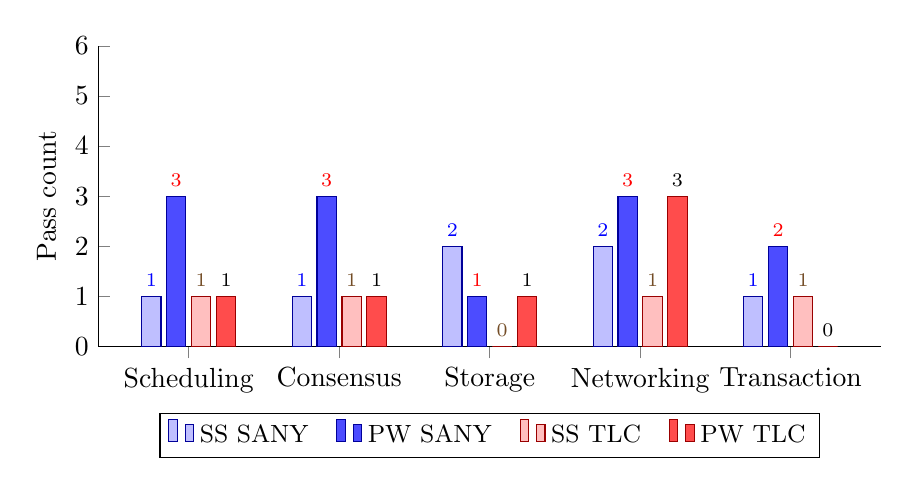
\begin{tikzpicture}
\begin{axis}[
  width=0.95\linewidth, height=5.4cm,
  ybar=2pt, bar width=7pt,
  enlarge x limits=0.15,
  ylabel={Pass count},
  symbolic x coords={Scheduling, Consensus, Storage, Networking, Transaction},
  xtick=data,
  ymin=0, ymax=6,
  ytick={0,1,2,3,4,5,6},
  legend style={at={(0.5,-0.22)}, anchor=north, legend columns=4,
    /tikz/every even column/.append style={column sep=8pt}, font=\small},
  nodes near coords, nodes near coords style={font=\scriptsize},
  axis lines*=left,
]
\addplot+[fill=blue!25, draw=blue!60!black] coordinates
  {(Scheduling,1) (Consensus,1) (Storage,2) (Networking,2) (Transaction,1)};
\addplot+[fill=blue!70, draw=blue!60!black] coordinates
  {(Scheduling,3) (Consensus,3) (Storage,1) (Networking,3) (Transaction,2)};
\addplot+[fill=red!25, draw=red!60!black] coordinates
  {(Scheduling,1) (Consensus,1) (Storage,0) (Networking,1) (Transaction,1)};
\addplot+[fill=red!70, draw=red!60!black] coordinates
  {(Scheduling,1) (Consensus,1) (Storage,1) (Networking,3) (Transaction,0)};
\legend{SS SANY, PW SANY, SS TLC, PW TLC}
\end{axis}
\end{tikzpicture}
\caption{Per-domain pass counts for single-shot (SS) vs.\ piecewise (PW)
on each verifier level. The piecewise pipeline never increases TLC pass
on scheduling, consensus, or transaction; its entire $+2$ TLC delta is
located in the storage and networking columns. The transaction bar shows
the only TLC regression: a single problem (Two-Phase Commit) drops from
pass to fail under piecewise. The chart makes it visually clear that
``piecewise dominates single-shot'' is not what the data show.}
\label{fig:domain-bars}
\end{figure}

\paragraph{Why the SANY pass rate moves more than the TLC pass rate.}
SANY rises by $5$ problems under piecewise; TLC rises by only $2$. This
is the expected shape if decomposition is helping the model write
syntactically well-formed modules but is not yet helping it write
modules with non-trivial state graphs. The four difficulty-$4$ problems
that go from SANY-fail under single-shot to SANY-pass under piecewise
all then fail TLC, illustrating the same pathology the Diamond audit
exposes in the labelled corpora: improving the parser-acceptance signal
without improving the state-space signal merely moves spec generation
into the parser-clean-but-vacuous regime, rather than into the
mutation-sensitive regime we actually want.

% ---------------------------------------------------------------------------
\section{Discussion}
\label{sec:discussion}

\paragraph{What the audit means in practice.} The Diamond audit
(\S\ref{sec:diamond}) does \emph{not} say that previously labelled gold specs
are syntactically broken---they all pass SANY---but rather that they cannot
distinguish a working model checker from a check that has nothing to check.
For an LLM training pipeline this matters because the gradient signal sent by
those examples is, in expectation, an instruction to write smaller and quieter
specifications. We observed this empirically across several rounds of
preference-optimisation training (KTO, DPO) before discovering the underlying
labelling defect: each round nominally improved the binary
\texttt{tlc\_pass} metric while monotonically degrading the qualitative
fidelity of the produced specs.

\paragraph{Verifiers as inference-time, not training-time, signal.} The
piecewise result (\S\ref{sec:piecewise}) suggests an inversion of the usual
ordering. Rather than spending compute distilling the verifier signal into
model weights, we use the verifier directly at inference time, on small
artefacts where its feedback is structurally local. The model's job becomes
producing five short candidates and repairing them on demand; the verifier
does the work of selecting which candidates survive. This is closer in spirit
to constraint-guided search than to fine-tuning.

\paragraph{When fine-tuning is still useful.} Decomposition is not a substitute
for domain knowledge. The remaining benchmark failures are problems where the
model does not know what the right \texttt{Next} actions \emph{are}---no amount
of repair will produce a Chandy--Lamport snapshot from a model that has never
seen one. The constructive next step is to use the piecewise pipeline as a
\emph{data generator}, producing Diamond-passing examples for those domains
specifically and feeding them back into a small, targeted SFT run. We expect
this kind of pipeline (verifier-curated, decomposition-generated, narrowly
scoped fine-tuning) to be more effective per FLOP than broad-corpus training.

\paragraph{Limitations.}
\emph{Benchmark size and authorship.} The benchmark is small ($n=20$) and
authored by us. Five additional successes drive the headline claim, and we
do not report variance across seeds: every cell in
Tables~\ref{tab:headline} and~\ref{tab:domain} is a single run, and
informal repeats of the single-shot pipeline suggest a $\pm 1$--$2$
problem-level wobble around the reported numbers. The $1/20 \to 6/20$ gap
is large enough to survive that wobble qualitatively, but we do not claim a
quantitatively precise effect size, and a multi-seed replication is the
single most important follow-up. The self-authored benchmark also creates a
selection-bias risk: our choice of problems shapes which failure modes are
visible, and the difficulty of e.g.\ Chandy--Lamport may be a property of
how we phrased that problem rather than a general statement about the
method's reach. We chose the 20 problems before running either pipeline and
froze them, but a third-party benchmark would be a strictly stronger test
and is the obvious target for follow-on work.

\emph{Diamond gate.} The Diamond gate is a sufficient condition for
non-trivial behaviour, not a complete characterisation of specification
quality; a Diamond-passing spec can still be wrong with respect to the
user's intent. Mutation testing is sensitive to the specific mutation
operators chosen; we use only two phases here, and a stronger gate is
plausible. Our worked-example inspection (\S\ref{sec:diamond}) suggests
the gate is not over-rejecting on the failure samples we examined, but a
larger manual audit would tighten that claim.

\emph{Single model.} All experiments use one underlying checkpoint
(\texttt{gpt-oss:20b}). We do not yet know whether the piecewise gain
generalises to coding-specialised 20Bs or to substantially larger models.

\emph{Missing best-of-$N$ control.} The piecewise pipeline averages
$5.5$ verifier-validated attempts per problem, against single-shot's
$1$. The fair compute-matched baseline is best-of-$5$ or best-of-$15$
single-shot with the same verifier as oracle, and we do not yet have
that number. The honest reading of Table~\ref{tab:headline} is therefore
that piecewise produces a $+2$ TLC and $+5$ SANY improvement \emph{at
$\geq 5\times$ compute}, and the share of that gain attributable to
decomposition (as opposed to additional verifier rolls) is currently
unknown. An earlier draft of this paper described the headline as a
``$6\times$ improvement''; we have removed that framing because it relied
on a $1/20$ single-shot baseline that does not match
\texttt{outputs/benchmark\_results.csv}, and because the matched-compute
control is missing.

\emph{Per-problem regressions.} Two single-shot TLC successes
(\texttt{BM002} Two-Phase Commit, \texttt{BM011} Paxos Single-Decree)
are lost under piecewise, and two single-shot SANY-clean specs
(\texttt{BM010} KV Store, \texttt{BM020} Eventually Consistent Counter)
become SANY-broken. We did not anticipate these regressions and we do
not have a clean explanation for them; the working hypothesis is that
the per-piece decomposition removes contextual information that
tightly-coupled small specifications need
(\S\ref{sec:challenges}).

\paragraph{Reproducibility.} The Diamond gate, the audit script, and the
piecewise generation pipeline are implemented in
\texttt{src/validators/tlc\_validator.py},
\texttt{scripts/audit\_fm\_alpaca.py}, and
\texttt{src/inference/piecewise\_gen.py} respectively. The benchmark
problems and per-problem CSV outputs are in
\texttt{outputs/benchmark\_results/}. All results in this paper can be
regenerated from a single \texttt{ollama} model checkpoint and a local TLA
toolbox.

% ---------------------------------------------------------------------------
\section{Conclusion}

The bottleneck in LLM-driven TLA\textsuperscript{+} authoring is not the
model's grammar---a mid-sized open model can already write
TLA\textsuperscript{+} that parses---but the discipline of the verifier
signal it is asked to optimise. We have argued, with two pieces of evidence,
that a sharper verifier is more valuable than more data: the Diamond audit
shows that current corpora cannot tell trivial from non-trivial behaviour,
and the piecewise generation result shows that a $+5$ SANY and $+2$ TLC
improvement on a 20-problem benchmark is available simply by giving the
verifier smaller artefacts to look at, with no change in model weights---at
the cost of a $\geq 5\times$ inference budget and a small number of
per-problem regressions on tightly-coupled consensus specifications. The
constructive position is that future work in this area should treat the
verifier as a first-class element of the inference procedure, and reserve
training compute for the narrow domains where decomposition alone runs out
of model knowledge.

% ---------------------------------------------------------------------------
\section*{Acknowledgements}
\textit{(to be filled in)}

% ---------------------------------------------------------------------------
\bibliographystyle{plain}
\begin{thebibliography}{99}

\bibitem{lamport2002specifying}
Leslie Lamport.
\newblock \emph{Specifying Systems: The TLA\textsuperscript{+} Language and
Tools for Hardware and Software Engineers}.
\newblock Addison-Wesley, 2002.

\bibitem{newcombe2015use}
Chris Newcombe, Tim Rath, Fan Zhang, Bogdan Munteanu, Marc Brooker, and
Michael Deardeuff.
\newblock How Amazon Web Services uses formal methods.
\newblock \emph{Communications of the ACM}, 58(4):66--73, 2015.

\bibitem{andrews2005mutation}
James H. Andrews, Lionel C. Briand, and Yvan Labiche.
\newblock Is mutation an appropriate tool for testing experiments?
\newblock In \emph{ICSE}, 2005.

\bibitem{jiang2023draft}
Albert Q. Jiang, Sean Welleck, Jin Peng Zhou, Wenda Li, Jiacheng Liu,
Mateja Jamnik, Timoth\'ee Lacroix, Yuhuai Wu, and Guillaume Lample.
\newblock Draft, Sketch, and Prove: Guiding formal theorem provers with
informal proofs.
\newblock In \emph{International Conference on Learning Representations
(ICLR)}, 2023.

\bibitem{spencer2026canllms}
Eric Spencer.
\newblock Can LLMs write correct TLA\textsuperscript{+} specifications?
Evaluating natural-language-to-TLA\textsuperscript{+} generation.
\newblock Manuscript, 2026.

\bibitem{fmalpaca}
FM-Universe.
\newblock FM-Alpaca: An instruction-tuning dataset for formal methods.
\newblock Hugging Face dataset, \texttt{fm-universe/FM-alpaca}, 2024.

\bibitem{misu2024towards}
Md Rakib Hossain Misu, Cristina V. Lopes, Iris Ma, and James Noble.
\newblock Towards AI-assisted synthesis of verified Dafny methods.
\newblock \emph{Proceedings of the ACM on Software Engineering}, 1(FSE), 2024.

\bibitem{first2023baldur}
Emily First, Markus N. Rabe, Talia Ringer, and Yuriy Brun.
\newblock Baldur: Whole-proof generation and repair with large language models.
\newblock In \emph{Proceedings of the 31st ACM Joint European Software
Engineering Conference and Symposium on the Foundations of Software
Engineering (ESEC/FSE)}, 2023.

\end{thebibliography}

\end{document}
